\section{Data Acquisition}

%head
The following section will include a description on how the data for the study have been acquired and processed. All data processing, along with GUI design and implementation will be done in Matlab.

%presentaion of training GUI
To acquire data a training GUI has been designed and implemented in Matlab. The GUI has been designed to fulfil the specific needs for this project, but with the fact in mind that it could be modulated for future use. A picture of the GUI can be seen in \figref{fig:GUI_Training}. 




\begin{figure}[H]
	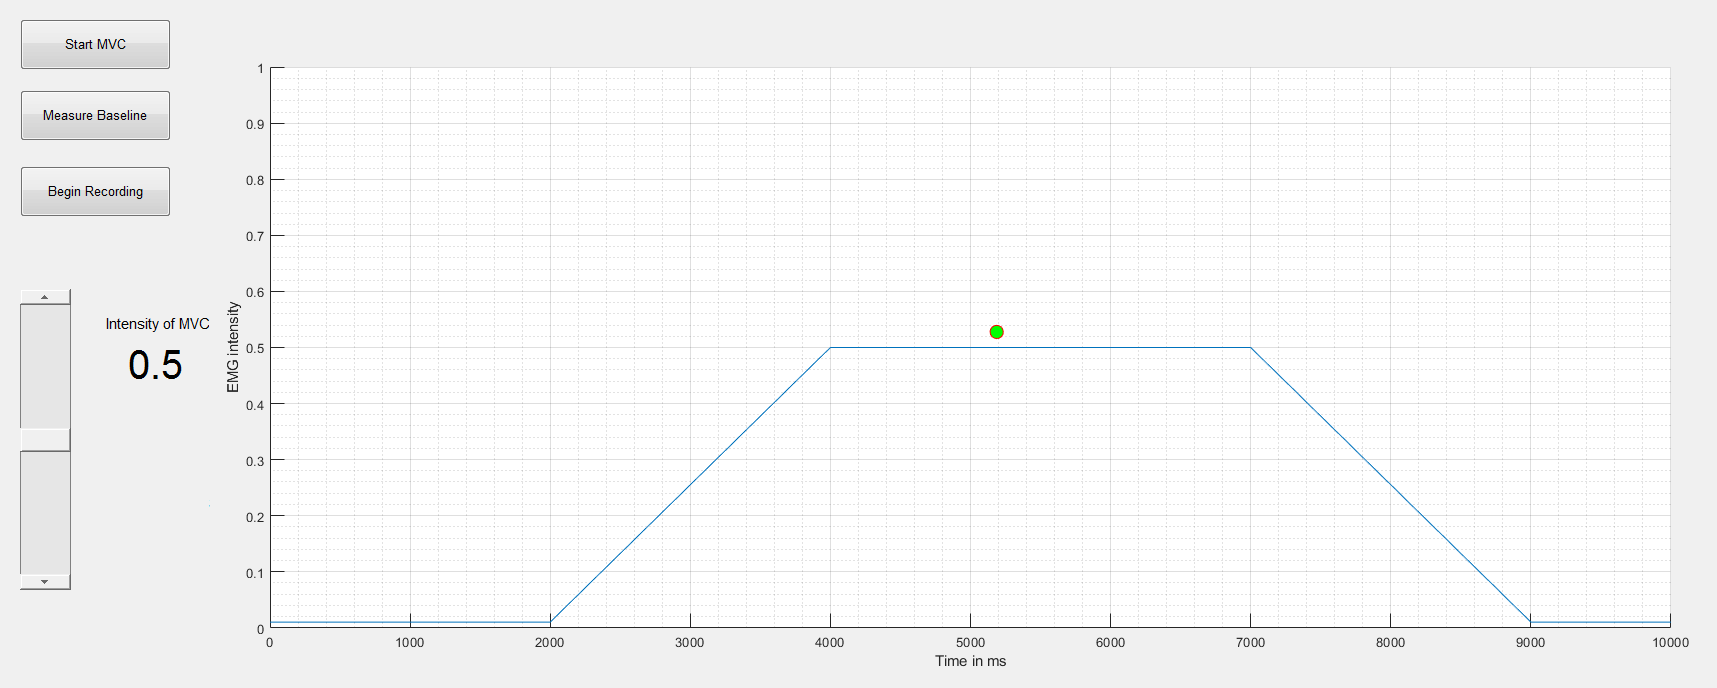
\includegraphics[width=.4\textwidth]{figures/GUI/GUI_Training.png}  %<--but is not needed.
	\caption{The training GUI implemented with Matlab. Control buttons to calculate MVC and perform MVC fraction recordings are on the left. The trapezoid plot with the yellow dot controlled by the recorded EMG from the test subejct, shown on the right. The fraction of the MVC can be defined by the slider located under the control bottons.}
	\label{fig:GUI_Training}
\end{figure} 




%presentation of acquired data




